
\documentclass[10pt,openany,a4paper]{article}
\usepackage{tikz, pgfplots, tkz-euclide,calc}
\usetikzlibrary{patterns,shapes.arrows,calc}
\usepackage{fancyhdr}
\usepackage{enumerate,enumitem}
\usepackage{cancel}
\usepackage{varwidth}

% TAMBAHKAN PACKAGE SENDIRI KALAU KURANG

\usepackage{geometry}
\geometry{
	left = 22mm,
	right = 22mm,
	top = 25mm,
	bottom = 25mm,
}
\usepackage{graphicx}
\usepackage{subcaption}
\usepackage{soul}
\usepackage{hyperref}
\usepackage{float}
\usepackage{setspace}
\usepackage{afterpage}
\usepackage{xcolor}
\usepackage[nosectionbib]{apacite}
\usepackage{lmodern}
\usepackage{mathtools}
\usepackage{upgreek}
\usepackage{siunitx}
% \usepackage{fontawesome5}
\usepackage{fontawesome6}
\usepackage{physics}
\usepackage{pdfpages}
\usepackage{hyperref}
\renewcommand{\baselinestretch}{1.3}
\usepackage{multicol}
\usepackage{hyperref,ragged2e,amsmath,multicol,gensymb,setspace,
fancyhdr,amsfonts,tikz,pgfplots,nccmath,enumerate,verbatim,amsthm,physics}
\usepgfplotslibrary{polar,fillbetween}
% Disable tikz externalization to avoid requiring -shell-escape
\usepgfplotslibrary{external}
\tikzexternalize[prefix=tikz/]
\tikzset{reuse path/.code={\pgfsyssoftpath@setcurrentpath{#1}}}
\usetikzlibrary{shapes.geometric,arrows}
\newcommand\mylog[1]{\mathop{{}^{#1}\mathrm{log}}}
\pgfplotsset{compat=1.15}
\pgfplotsset{my style/.append style={axis x line=middle, axis y line=
middle, xlabel={$x$}, ylabel={$y$}, axis equal }}
\usepackage{etoolbox}
% remove stray \makeatother
\newtheorem{defn}{Definisi}[section]
\newtheorem{teo}[defn]{Teorema}
\newtheorem{thm}{Teorema}[section]
\newtheorem{lemma}{Lemma}
\newtheorem{lemmas}[defn]{Lemma}
\newtheorem{cor}[defn]{Akibat}
\newtheorem{asumsi}[defn]{Asumsi}
\theoremstyle{definition}
\newtheorem{con}{Contoh}[section]
\theoremstyle{definition}
\theoremstyle{plain}
\newtheorem{prop}{Proposisi}[section]
\renewcommand{\proofname}{Bukti}
\renewcommand{\thethm}{\arabic{chapter}.\arabic{thm}}

\newcommand{\normlp}[1]{\left\|#1\right\|_{L^p_{\lambda}(0,T;H)}}% Fungsi norm (||x||)
\newcommand{\R}{\mathbb{R}}
\renewcommand{\natural}{\mathbb{N}}
\newcommand{\Xpl}{X^R_{p,\lambda}}
\newcommand{\Xpls}{X^R_{p,\lambda^*}}
\newcommand{\qpl}{q^R_{p,\lambda}}
\newcommand{\qpls}{q^R_{p,\lambda^*}}
\pagestyle{fancy}
\fancyhf{}
\lhead{Halaman \thepage}
% \cfoot{\faXTwitter\ \href{https://x.com/ahmadzakiyudin_/}{@ahmadzakiyudin\_} | \faInstagram\ \href{https://instagram.com/ahmadzakiyudin_/}{@ahmadzakiyudin\_} | \faTiktok\ \href{https://tiktok.com/@ahmathz/}{@ahmathz}}
% \rhead{Pembahasan Soal ETS \\ Kalkulus 1 ITS 2025/2026}
\hypersetup{
    colorlinks=true,
    linkcolor=blue,
    filecolor=blue,      
    urlcolor=blue,
}
\newenvironment{jawab}[2][tes]{
% \fbox{\begin{minipage}{14.65cm}
\textbf{Kata kunci materi:} #1.\\
\textbf{Penyelesaian:} #2
% \end{minipage}}
}{}

\newenvironment{jawab2}[2][tes]{
\fbox{\begin{minipage}{14.65cm}
 #2
\end{minipage}}}{}

\newenvironment{jawaban}[2][tes]{
\colorlet{oldcolor}{.}
        \color{red}
        \setlength{\fboxrule}{1pt}\boxed{\color{oldcolor}#2}\color{oldcolor}.
}{}

\newenvironment{jawaban2}[2][tes]{
\colorlet{oldcolor}{.}
        \color{red}
        \setlength{\fboxrule}{1pt}\fbox{\color{oldcolor}#2}\color{oldcolor}.
}{}

\newenvironment{penting}[2][tes]{
\colorlet{oldcolor}{.}
\color{blue}
\fbox{\color{oldcolor}#2}\color{oldcolor}
}{}

\begin{document}
% \begin{titlepage}
%     \vspace*{\fill}
%     \begin{center}
%       \Huge {PEMBAHASAN SOAL EAS \\ KALKULUS II \\ TAHUN 2024/2025}\\[0.4 cm]
%       \huge {Ahmad Hisbu Zakiyudin}\\[0.2 cm]
%       \Large {(\href{https://instagram.com/ahmadzakiyudin_/}{@ahmadzakiyudin\_})}
%     \end{center}
%     \vspace*{\fill}
%   \end{titlepage}
% !TEX root = ../../BookTemplate.tex
%%%%%%%%%%%%%%%%%%%%%%%%%%%%%%%%%%%%%%%%%%%%%%%%%%%%%%%%%%%%%%%%%%%%%%%%%%%%%%%%%%
% \begin{titlepage}
%     \raggedleft	
% 	\hspace{.025\textwidth}
% 	\parbox[b]{\textwidth}{
%     \vspace{1.5cm}
% 		{\Huge\bfseries Pembahasan Soal EAS}                \\[20pt]
% 		{\huge\textit\ Kalkulus II}\\ \\[10pt]
%         {\Large\textsc{Tahun 2024/2025}}}
% \vfill
% \rule{1pt}{.14\textheight}
% \hspace{.025\textwidth}
%     \raisebox{10pt}{\parbox[b]{.95\textwidth}{ 
%         {\Large\textsc{Ahmad Hisbu Zakiyudin}}              \\[10pt]
%         \large{\href{https://instagram.com/ahmadzakiyudin_/}{@ahmadzakiyudin\_}}               \\[25pt]
%         {\large 5 Juni 2026}}}
% \end{titlepage}
\begin{titlepage}
	\centering % Center everything on the title page
	% \scshape % Use small caps for all text on the title page
	\vspace*{1.5\baselineskip} % White space at the top of the page
% ===================
%	Title Section 	
% ===================

	\rule{13cm}{1.6pt}\vspace*{-\baselineskip}\vspace*{2pt} % Thick horizontal rule
	\rule{13cm}{0.4pt} % Thin horizontal rule
	
		\vspace{0.75\baselineskip} % Whitespace above the title
% ========== Title ===============	
	{	\Huge Pembahasan Soal ETS\\ 
			\vspace{4mm}
		Kalkulus 1 \\ \vspace{2mm} \huge{Tahun 2024/2025}\\	}
% ======================================
		\vspace{0.75\baselineskip} % Whitespace below the title
	\rule{13cm}{0.4pt}\vspace*{-\baselineskip}\vspace{3.2pt} % Thin horizontal rule
	\rule{13cm}{1.6pt} % Thick horizontal rule
	
		\vspace{1.75\baselineskip} % Whitespace after the title block
% =================
%	Information	
% =================
{\large Oleh: Ahmad Hisbu Zakiyudin}
	% {\large Oleh: Ahmad Hisbu Zakiyudin \\
	% 	\vspace*{1.2\baselineskip}
	% \href{https://instagram.com/ahmadzakiyudin_/}{@ahmadzakiyudin\_}} \\
	\vfill
	\vspace{1mm}
\huge{Selamat Belajar!}
\end{titlepage}
\makeatletter
\setlength\fboxsep{3pt}
% ensure enough header height for fancyhdr
\setlength{\headheight}{24pt}
 \begin{center}
	{\underline{\textbf{\MakeUppercase{Soal dan Pembahasan ETS Matematika Tahun 2024/2025}}}}
    \end{center}

    \begin{center}
	\begin{tabular}{lcl}
		Mata kuliah/SKS & : & Matematika ( SM234152 ) / 2 SKS\\
		Hari, Tanggal & : & Senin, 14 Oktober 2024\\
		Waktu & : & 11.00 - 12.40 / 100 menit\\
		Sifat & : & Tertutup\\
		Kelas & : & 1-7\\
  ~
	\end{tabular}

    \noindent\rule{\textwidth}{2.pt}
        \end{center}
\begin{enumerate}
    \item Dapatkan himpunan penyelesaian dari $\dfrac{1}{x+1}>\dfrac{1}{x-3}$.

    \item Diketahui garis $l_1$ melalui titik $(1,3)$ dan $(3,7)$. Dapatkan persamaan garis $l_2$ yang melalui titik $(4,5)$ dan tegak lurus dengan garis $l_1$.

    \item Selesaikan sistem persamaan linear berikut menggunakan metode eliminasi Gauss-Jordan:
    \begin{align*}
        x-y+2z &= 4\\
        2x+y+z &= 5\\
        3x-y+2z &= 6
    \end{align*}

    \item Diketahui fungsi $f(x)=-x^2-2x+3$.
    \begin{enumerate}
        \item Dapatkan domain dan range dari $f(x)$.
        \item Sketsa grafik $f(x)$.
    \end{enumerate}

    \item Diberikan sistem persamaan fungsi permintaan dan penawaran
    \begin{align*}
        2P &= -Q_d+125\\
        8P &= Q_s+45
    \end{align*}
    dengan $P,Q_d,Q_s$ masing-masing adalah harga, jumlah permintaan, dan jumlah penawaran.
    \begin{enumerate}
        \item Tentukan harga dan jumlah barang di titik equilibrium.
        \item Misalkan pemerintah memberikan pajak sebesar 2 untuk masing-masing barang. Tentukan persamaan fungsi permintaan dan penawaran setelah dikenakan pajak dan pembagian pembayaran pajaknya!
    \end{enumerate}
\end{enumerate}
\newpage
 \begin{center}
	{\underline{\textbf{\MakeUppercase{Soal dan Pembahasan ETS Kalkulus 1 Tahun 2024/2025}}}}
    \end{center}

    \begin{center}
	\begin{tabular}{lcl}
		Mata kuliah/SKS & : & Kalkulus 1 ( SM234101 ) / 3 SKS\\
		Hari, Tanggal & : & Rabu, 16 Oktober 2024\\
		Waktu & : & 07.00 - 08.40 / 100 menit\\
		Sifat & : & Tertutup\\
		Kelas & : & 13-19, 103\\
  ~
	\end{tabular}

    \noindent\rule{\textwidth}{2.pt}
        \end{center}
    \begin{enumerate}
    \item Diberikan titik $A(2,-1)$, $B(2,2)$ dan $C(0,4)$. Dapatkan persamaan garis yang melalui titik $A$ dan sejajar dengan garis yang melalui $B$ dan $C$.

    \item Diberikan $f(x)=\dfrac{1}{x^2-4}$ dan $g(x)=\sqrt{x+1}$.
    \begin{enumerate}
        \item Dapatkan domain $f(x)$ dan $g(x)$.
        \item Dapatkan $(f\circ g)(x)$ dan domain $(f\circ g)(x)$.
    \end{enumerate}

    \item Diberikan $f(x)=x^2-4x+7$.
    \begin{enumerate}
        \item Tentukan domain dari $f$ sehingga $f^{-1}$ ada.
        \item Dapatkan $f^{-1}$ beserta domainnya.
    \end{enumerate}

    \item Dapatkan nilai $k$ sedemikian sehingga fungsi:
    \begin{align*}
        f(x)=\begin{cases}
            x^2-k, & x<3\\
            3x-3, & x\geq 3.
        \end{cases}
    \end{align*}
    kontinu di $x=3$.

    \item Dapatkan $f'(x)$ dimana $f(x)=\sqrt{\dfrac{(3x+1)^3}{2x}}$.
\end{enumerate}
\newpage
 \begin{center}
	{\underline{\textbf{\MakeUppercase{Soal dan Pembahasan ETS Kalkulus 1 Tahun 2024/2025}}}}
    \end{center}

    \begin{center}
	\begin{tabular}{lcl}
		Mata kuliah/SKS & : & Kalkulus 1 ( SM234101 ) / 3 SKS\\
		Hari, Tanggal & : & Kamis, 17 Oktober 2024\\
		Waktu & : & 07.00 - 09.40 / 100 menit\\
		Sifat & : & Tertutup\\
		Kelas & : & 5-12, 101\\
  ~
	\end{tabular}

    \noindent\rule{\textwidth}{2.pt}
        \end{center}
    \begin{enumerate}
    \item Dapatkan himpunan penyelesaian dari $\dfrac{1}{x+2}<\dfrac{1}{4-x}$.

    \item Diberikan $f(x)=x^2+2,\ x\geq 0$ dan $g(x)=\sqrt{x-3}$.
    \begin{enumerate}
        \item Dapatkan domain $f(x)$ dan $g(x)$.
        \item Dapatkan $(g\circ f)(x)$ dan domain $(g\circ f)(x)$.
    \end{enumerate}

    \item Diketahui $f(x)=x^3-2$.
    \begin{enumerate}
        \item Dapatkan $f^{-1}(x)$ beserta domainnya.
        \item Sketsa grafik dari $f(x)$ dan $f^{-1}(x)$ pada satu bidang koordinat.
    \end{enumerate}

    \item Hitunglah $\displaystyle\lim_{x\to-\infty}\frac{\sqrt{5x^2-2}}{x+3}$.

    \item Dapatkan persamaan garis singgung kurva $xy^2+y+\sqrt{x}=x+3$ di titik $(4,1)$.
\end{enumerate}
\newpage
 \begin{center}
	{\underline{\textbf{\MakeUppercase{Soal dan Pembahasan ETS Kalkulus 1 Tahun 2024/2025}}}}
    \end{center}

    \begin{center}
	\begin{tabular}{lcl}
		Mata kuliah/SKS & : & Kalkulus 1 ( SM234101 ) / 3 SKS\\
		Hari, Tanggal & : & Kamis, 17 Oktober 2024\\
		Waktu & : & 09.00 - 10.40 / 100 menit\\
		Sifat & : & Tertutup\\
		Kelas & : & 47-59, 111\\
  ~
	\end{tabular}

    \noindent\rule{\textwidth}{2.pt}
        \end{center}
    \begin{enumerate}
    \item Dapatkan himpunan penyelesaian dari $\dfrac{1}{|2x-5|}>5$.

    \item Diberikan $f(x)=\sqrt{x-3}$ dan $g(x)=1+\sqrt{x-5}$.
    \begin{enumerate}
        \item Dapatkan domain $f(x)$ dan $g(x)$.
        \item Dapatkan $(f\circ g)(x)$ dan domain $(f\circ g)(x)$.
    \end{enumerate}

    \item Diberikan $f(x)=\sqrt[3]{x-1},\ x\geq 1$.
    \begin{enumerate}
        \item Dapatkan $f^{-1}(x)$ beserta domainnya.
        \item Sketsa $f(x)$ dan $f^{-1}(x)$ pada satu bidang koordinat.
    \end{enumerate}

    \item Hitunglah $\displaystyle\lim_{y\to-\infty}\frac{2-y}{\sqrt{7+4y^2}}$.

    \item Dapatkan persamaan garis singgung kurva $x^2+y+\dfrac{y}{x}=\sqrt{x}+2$ di titik $(1,1)$.
\end{enumerate}
\newpage
 \begin{center}
	{\underline{\textbf{\MakeUppercase{Soal dan Pembahasan ETS Kalkulus 1 Tahun 2024/2025}}}}
    \end{center}

    \begin{center}
	\begin{tabular}{lcl}
		Mata kuliah/SKS & : & Kalkulus 1 ( SM234101 ) / 3 SKS\\
		Hari, Tanggal & : & Kamis, 17 Oktober 2024\\
		Waktu & : & 11.00 - 12.40 / 100 menit\\
		Sifat & : & Tertutup\\
		Kelas & : & 20-33, 105, 106\\
  ~
	\end{tabular}

    \noindent\rule{\textwidth}{2.pt}
        \end{center}
    \begin{enumerate}
    \item Dapatkan himpunan penyelesaian dari $-1\leq |2-x|<3$.

    \item Diberikan $f(x)=\sqrt{25-x^2}$ dan $g(x)=\dfrac{1}{x^2}$.
    \begin{enumerate}
        \item Dapatkan domain $f(x)$ dan $g(x)$.
        \item Dapatkan $(g\circ f)(x)$ dan domain $(g\circ f)(x)$.
    \end{enumerate}

    \item Diberikan $f(x)=\sqrt{4-x^2}$.
    \begin{enumerate}
        \item Tentukan domain dari $f(x)$ sehingga inversnya ada.
        \item Dapatkan $f^{-1}(x)$ beserta domainnya.
    \end{enumerate}

    \item Diberikan fungsi
    \begin{align*}
        f(x)=\begin{cases}
            \dfrac{4-x}{2-\sqrt{x}}, & x\neq 4\\
            6, & x=4
        \end{cases},
    \end{align*}
    Selidiki kekontinuan $f(x)$ di $x=4$.

    \item Dapatkan $f''(x)$ dimana $f(x)=2x+\left(2\sqrt{x}-3\right)^{-2}$.
\end{enumerate}
\newpage
 \begin{center}
	{\underline{\textbf{\MakeUppercase{Soal dan Pembahasan ETS Kalkulus 1 Tahun 2024/2025}}}}
    \end{center}

    \begin{center}
	\begin{tabular}{lcl}
		Mata kuliah/SKS & : & Kalkulus 1 ( SM234101 ) / 3 SKS\\
		Hari, Tanggal & : & Kamis, 17 Oktober 2024\\
		Waktu & : & 13.30 - 15.10 / 100 menit\\
		Sifat & : & Tertutup\\
		Kelas & : & 34-46, 107, 108\\
  ~
	\end{tabular}

    \noindent\rule{\textwidth}{2.pt}
        \end{center}
    \begin{enumerate}
    \item Diberikan titik $A(1,1)$, $B(4,2)$ dan $C(2,6)$. Tentukan jarak dari titik $C$ ke garis yang melalui titik $A$ dan $B$.

    \item Diberikan $f(x)=x-4$, untuk $x\geq 4$ dan $g(x)=\sqrt{4-x^2}$.
    \begin{enumerate}
        \item Dapatkan domain $f(x)$ dan $g(x)$.
        \item Tentukan $(g\circ f)(x)$ dan domain $(g\circ f)(x)$.
    \end{enumerate}

    \item Diberikan fungsi $f(x)=\sqrt{2x-x^2},\ 0\leq x\leq 1$.
    \begin{enumerate}
        \item Tentukan $f^{-1}(x)$ beserta domainnya.
        \item Gambarkan grafik $f(x)$ dan $f^{-1}(x)$ dalam satu bidang koordinat.
    \end{enumerate}

    \item Hitunglah $\displaystyle\lim_{x\to 2}\frac{\sqrt{x^2+5}-3}{x-2}$.

    \item Diketahui persamaan garis singgung kurva $y^2-xy=-2$ di titik $(a,b)$ sejajar dengan kurva $y=-x$. Dapatkan titik $(a,b)$.
\end{enumerate}

\newpage 

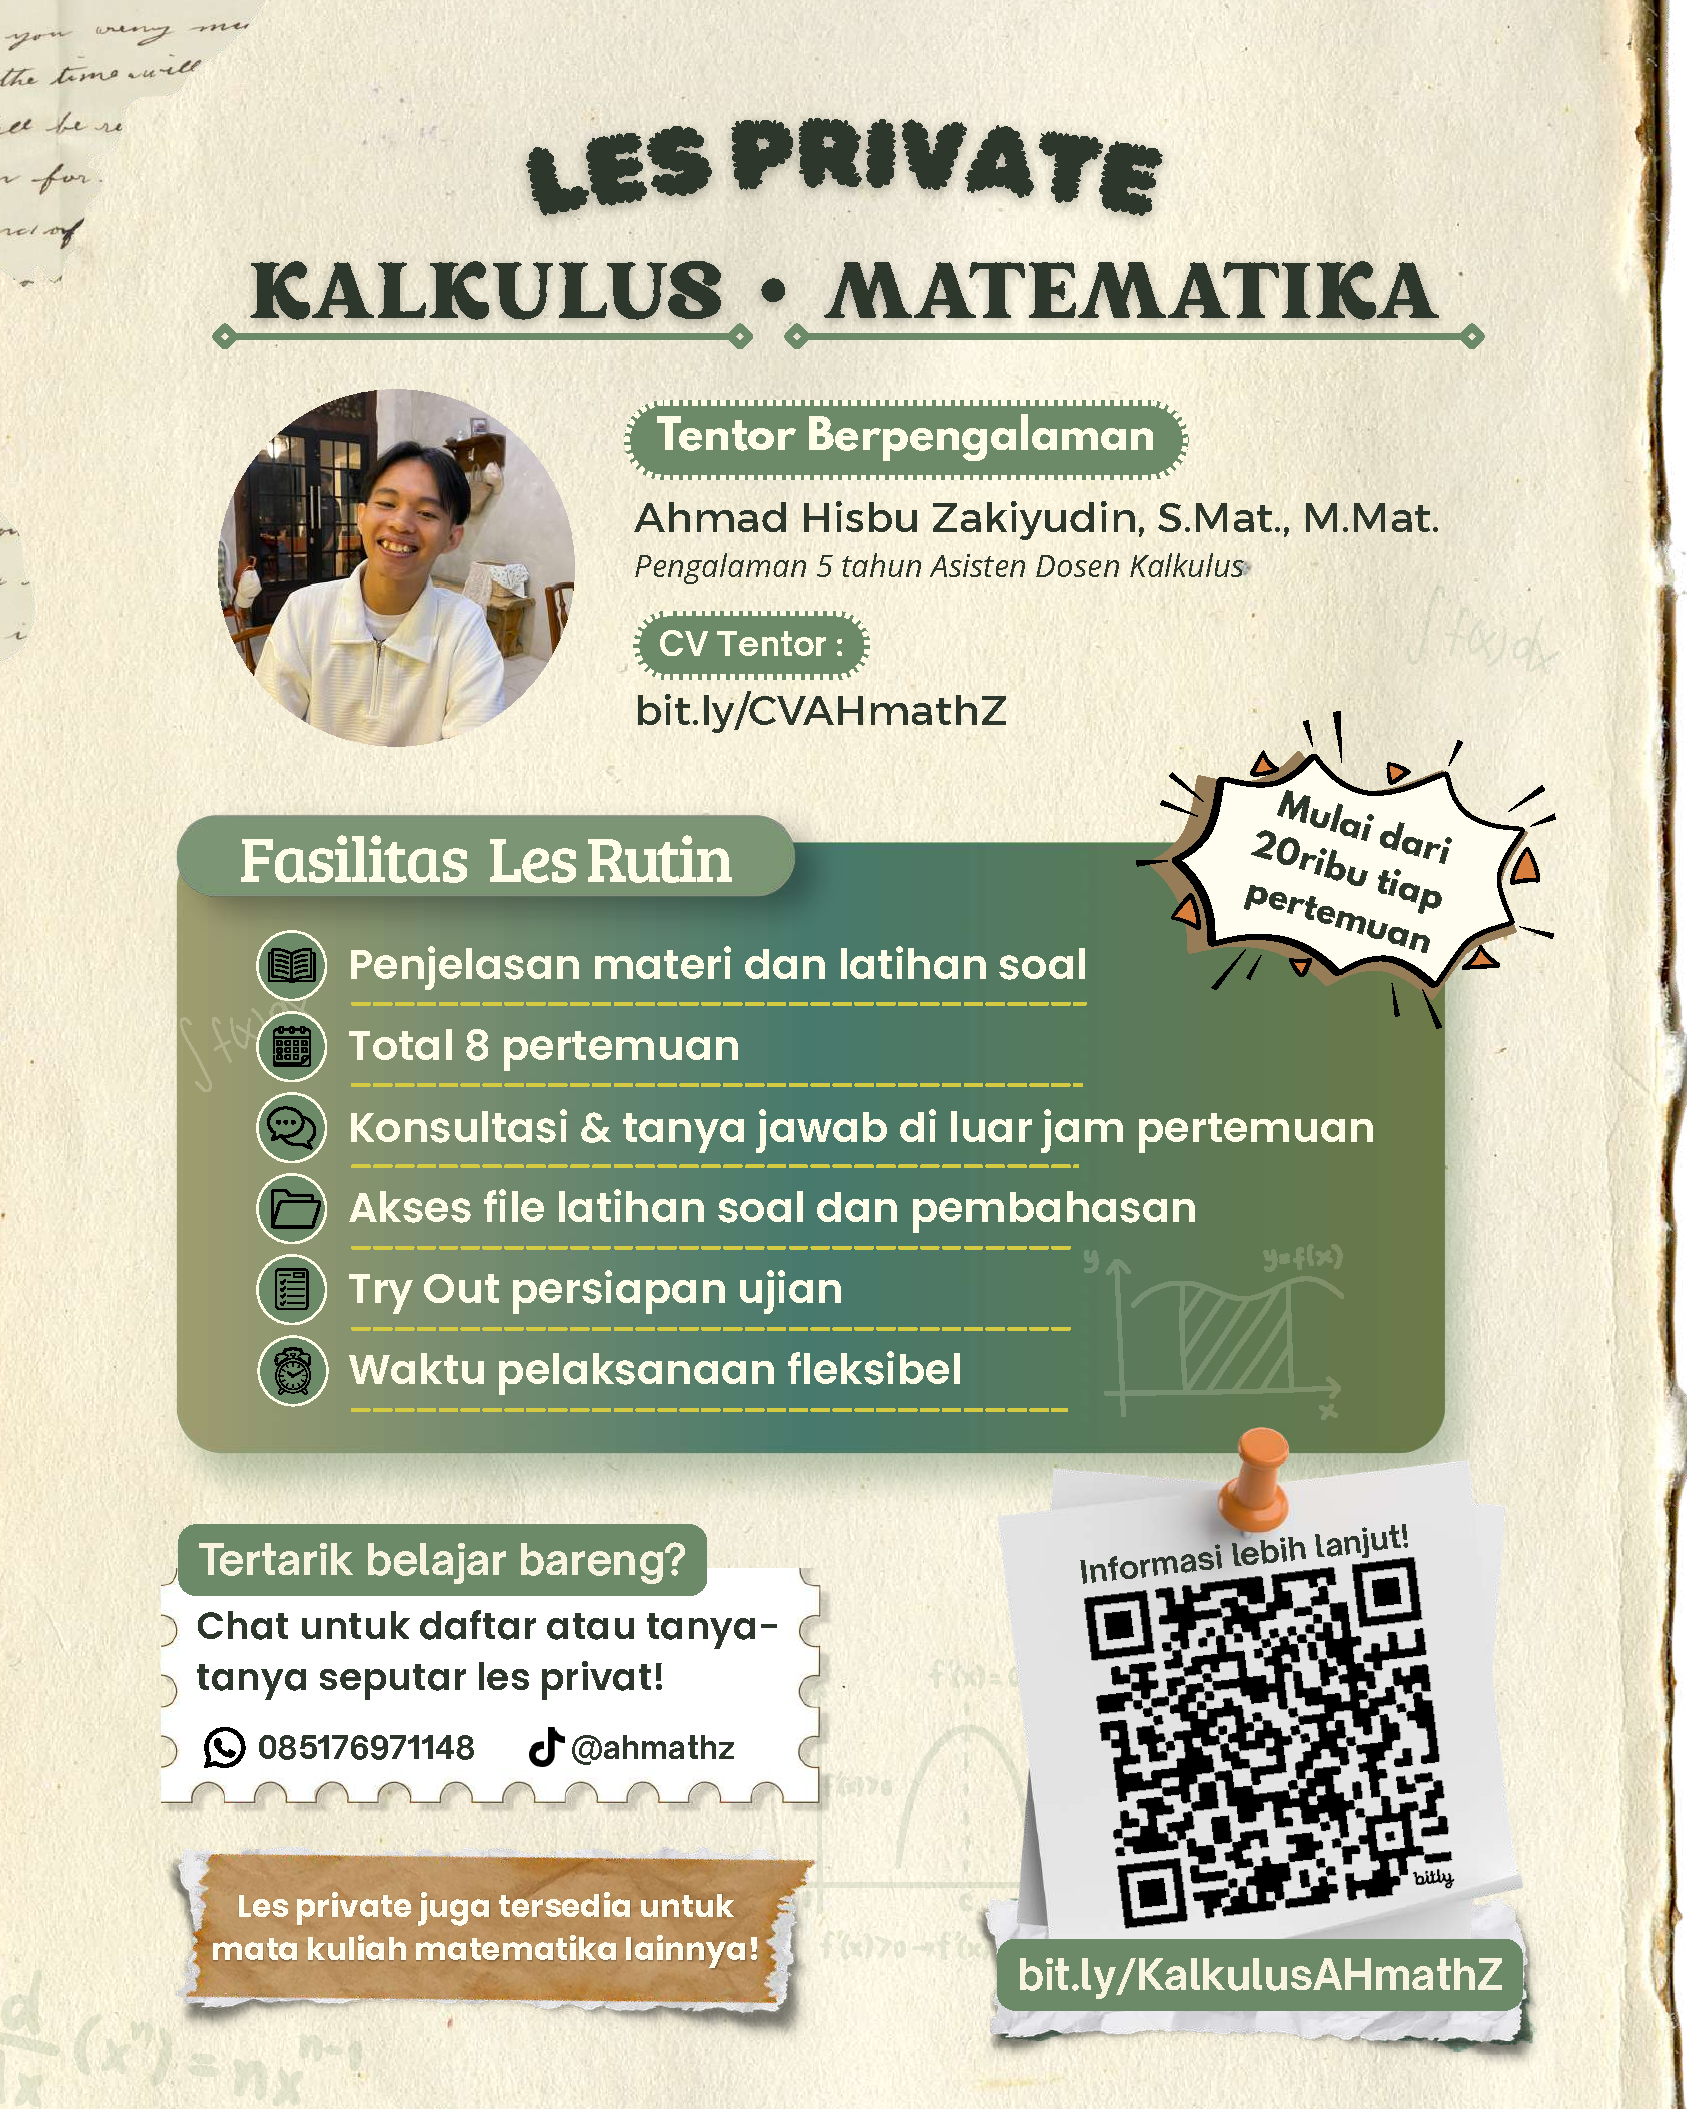
\includepdf[pages=-]{../2025-2026/les.pdf}

\end{document}
